\section{Automatic Nested Loop Acceleration Framework} \label{sec:acc-framework}
By using a regular SCGRA overlay built on top of the physical FPGA devices, 
we developed an automatic nested loop acceleration framework 
as shown in \figref{fig:auto-acc-framework}. The main goal of the  
framework is to provide a push-button solution to 
nested loop acceleration on a CPU-FPGA system. With high-level 
nested loop description and design constraints, the design parameters 
are customized specifically to an user application.  
When the optimized design parameters are available, 
SCGRA overlay based FPGA accelerator as well as the communication 
interface between host CPU and the accelerator can be generated. 
Finally, the generated FPGA accelerator and software will be 
compiled to the target CPU-FPGA system rapidly. 

\begin{figure}[tb]
\center{\includegraphics[width=0.55\linewidth]{auto-acc-framework}}
\caption{Automatic nested loop acceleration framework}
\label{fig:auto-acc-framework}
\end{figure}

\subsection{Typical SCGRA Overlay Based FPGA Accelerator}
\figref{fig:scgra-acc} shows the design of a typical SCGRA overlay 
based FPGA accelerator. In the accelerator, on-chip
memory i.e. IBuf and OBuf are used to buffer the communication 
data between the host CPU and 
the accelerator. A controller is also presented in hardware 
to control the operations of the accelerator as well as
memory transfers. The SCGRA, which is the kernel computation fabric,
consists of an array of PEs and it achieves the computation 
task through the distributed control words stored in each PE. The AddrBuf 
stores all the valid IO buffer accessing addresses of the DFG. 

\begin{figure}[tbh]
\center{\includegraphics[width=0.8\linewidth]{scgra-accelerator}}
\caption{SCGRA overlay based FPGA accelerator}
\label{fig:scgra-acc}
\end{figure}

\subsection{Loop Execution On SCGRA Overlay Based FPGA Accel.}
\figref{fig:group-dfg} illustrates how the loop is executed 
on the FPGA accelerator step by step. First of all, 
data flow graph (DFG) is extracted from the loop and then it 
is scheduled on to the SCGRA overlay based FPGA accelerator. 
Depending on how much the loop is unrolled and transformed 
to DFG, the DFG may be executed repeatedly until the end of 
the original loop. In addition, data transfers for 
multiple executions of the same DFG are batched into groups 
as shown in \figref{fig:group-dfg}. This technique is used to 
reduce the number of data transmission between host CPU and FPGA, 
which further helps to amortize the initial communication cost. 
On the other hand, it will also result in larger on-chip memory 
overhead. And we will rely on the customization framework to 
compromise this design choices. 

\begin{figure}[tb]
\center{\includegraphics[width=0.85\linewidth]{group-dfg}}
\caption{Loop, group and DFG. The loop will be divided into 
groups. Each group will be partially unrolled and the unrolled part will be 
translated to DFG. IO transmission between FPGA and host CPU is performed 
in the granularity of a group.}
\label{fig:group-dfg}
\end{figure}

\subsection{SCGRA Overlay Compilation Framework}
Combining the existing compilation techniques 
in \cite{ROB2014} and \cite{scgra-orig}, we built 
a high productivity compilation framework targeting 
nest loop acceleration using SCGRA overlay. The framework 
is presented in \figref{fig:detailed-compilation} and it 
basically consists of two compilation paths as identified 
in the figure. 

\begin{figure}[t]
\center{\includegraphics[width=0.9\linewidth]{detailed-compilation}}
\caption{A high productivity SCGRA compilation framework}
\label{fig:detailed-compilation}
\end{figure}

When a nested loop is initially compiled to the specified SCGRA overlay based accelerator, 
both design flows must be followed. The HDL model of the accelerator 
will be generated based on the specified parameters. Then the accelerator 
can be rapidly implemented using the technique in \cite{ROB2014} and 
an empty FPGA accelerator bitstream will be produced. Meanwhile, 
DFG will be generated according to the specified unrolling factor 
and then scheduled to the SCGRA overlay. 
After the scheduling, control words are extracted and they can 
further be integrated into the empty FPGA accelerator bitstream. 
Finally, FPGA accelerator bitstream that can be used for 
the loop acceleration is acquired. According to \cite{ROB2014}, 
this process is typically 20 times faster than a standard HDL 
compilation flow. 

When the nested loop is just slightly modified during the design iterations, 
the bitstream of the accelerator can be reused and we can simply follow 
the compilation flow marked with the green arrows. The compilation process 
is able to complete in a few seconds which is getting close to a 
software compilation.


